% ****** Start of file apssamp.tex ******
%
%   This file is part of the APS files in the REVTeX 4.1 distribution.
%   Version 4.1r of REVTeX, August 2010
%
%   Copyright (c) 2009, 2010 The American Physical Society.
%
%   See the REVTeX 4 README file for restrictions and more information.
%
% TeX'ing this file requires that you have AMS-LaTeX 2.0 installed
% as well as the rest of the prerequisites for REVTeX 4.1
%
% See the REVTeX 4 README file
% It also requires running BibTeX. The commands are as follows:
%
%  1)  latex apssamp.tex
%  2)  bibtex apssamp
%  3)  latex apssamp.tex
%  4)  latex apssamp.tex
%
\documentclass[%
 reprint,
superscriptaddress,
citeautoscript,
%groupedaddress,
%unsortedaddress,
%runinaddress,
%frontmatterverbose,
%preprint,
showpacs,
% preprintnumbers,
%nofootinbib,
%nobibnotes,
%bibnotes,
 amsmath,amssymb,
 aps,
% prx,
%pra,
 prb,
%rmp,
%prstab,
%prstper,
%floatfix,
longbibliography,
]{revtex4-1}

\usepackage{graphicx}% Include figure files
\usepackage{dcolumn}% Align table columns on decimal point
\usepackage{bm}% bold math
\usepackage{xcolor}
\usepackage{hyperref}% add hypertext capabilities
\usepackage{afterpage}
\usepackage{bbold}
%\usepackage[mathlines]{lineno}% Enable numbering of text and display math
%\linenumbers\relax % Commence numbering lines

\newcommand{\infint}[1]{\int\limits_{-\infty}^{\infty}{#1}}

\begin{document}

\title{Notes on numerical stabilization in determinant quantum Monte Carlo}% Force line breaks with \\

\author{Carsten Bauer}
\affiliation{Institute for Theoretical Physics, University of Cologne, 50937 Cologne, Germany}

\date{\today}% It is always \today, today,
             %  but any date may be explicitly specified

\begin{abstract}
In these notes we will empirically compare different matrix decompositions for use in numerical stabilization in many-body quantum Monte Carlo simulation, in particular when calculating equal time Green's functions. We will both benchmark their speed and accuracy. We will further show that special care has to be taken when calculating time-displaced Green's functions and will review a well-known but somewhat hard to find method for stabilizing the necessary inversion in this case. We will focus on and use the Julia programming language for all calculations. An implementation of all discussed methods is available in the open-source software library \href{http://github.com/crstnbr/StableDQMC.jl}{\texttt{StableDQMC.jl}}.
\end{abstract}


\maketitle

%\tableofcontents

\section{\label{sec:why}The issue}

\subsection{Determinant quantum Monte Carlo in a nutshell}

For the description of the DQMC algorithm\cite{Blankenbecler1981}, we consider a quantum field theory that can be split into a purely bosonic part $S_B$ and a part $S_F$, which comprises fermion kinetics $T$ and boson-fermion interactions $V$. An example is the famous Hubbard model after decoupling the on-site
interaction $U n_{i, \uparrow} n_{i, \downarrow}$ by means of a Hubbard-Stratonovich or Hirsch transformation in either the spin or charge channel \cite{Hirsch1983}. As per usual, the central quantity of interest is the partition function
%
\begin{equation}
\mathcal{Z} = \int D\left( \psi, \psi^\dagger, \phi \right) e^{-S_B - S_F} \,.
\end{equation}
%
The basic idea is to switch from the $d$ dimensional quantum theory to a $D = d + 1$ dimensional classical theory as in the path integral framework. The first step is to discretize, $\beta = M \Delta \tau$, and Trotter decompose the imaginary time $\tau$,
%
\begin{align}
	\mathcal{Z} &= \int D\phi \ e^{-S_B} \mathrm{Tr}{\left[\exp{\left( -\Delta\tau \sum_{l=1}^M \psi^\dagger \left[T + V_\phi\right] \psi \right)}\right]} \label{eq:discretizedpi} \,.
\end{align}
%
The exponential is then separated and the appearing commutator ignored which results in a systematic error of the order $\mathcal{O}\left(\Delta\tau^2\right)$,
\begin{align}
	e^{A + B} &\approx e^A e^B \quad \nonumber\\
	e^{-\Delta\tau (T + V)} &\approx e^{- \frac{\Delta\tau}{2}T} e^{-\Delta\tau V} e^{- \frac{\Delta\tau}{2}T} + \mathcal{O}\left(\Delta\tau^3\right), \nonumber\\
	\mathcal{Z} &= \int D\phi \ e^{-S_B} \mathrm{Tr}{\left[ \prod_{l=1}^{m} B_l \right]} + \mathcal{O}\left(\Delta\tau^2\right). \label{eq:Ztr}
\end{align}
%
Note that the potential part $e^{-\Delta\tau \psi^\dagger V_\phi \psi}$ in the time-slice propagators $B_l = e^{- \frac{\Delta\tau}{2}\psi^\dagger T \psi} e^{-\Delta\tau \psi^\dagger V_\phi \psi} e^{- \frac{\Delta\tau}{2}\psi^\dagger T \psi}$ depends on the boson $\phi$ due to the present fermion-boson coupling. Rewriting the trace in \eqref{eq:Ztr} as a determinant, an identity which can be proven \textcolor{red}{CITE}, yields the fundamental form
%
\begin{align}
	\mathcal{Z} &= \int D\phi \ e^{-S_B} \det{G_\phi^{-1}} + \mathcal{O}\left(\Delta\tau^2\right), \label{eq:DQMC}
\end{align}
%
where
\begin{align}
	G = \left( \mathbb{1} + B_M B_{M-1} \cdots B_1 \right)^{-1} \label{etgf}
\end{align}
is the equal-time Green's function.

Only under specific circumstances, such as the presence of a symmetry, can the integral kernel be safely be interpreted as a probability weight, as $G_\phi$ and its determinant are generally complex valued (\textit{sign problem}).

\subsection{Numerical instabilities - Model system}

We consider the following simple non-interacting model system in one dimension,
\begin{align}
	H = -t\sum_{\langle i,j \rangle} c_i^\dagger c_j + \mu \sum_i n_i \label{eq:model},
\end{align}
where we set the hopping amplitude to $t=-1$ and the chemical potential to $\mu=-0.1$.
%\begin{align}
%H = \left[
%\begin{array}{cccccccc}
%-0.1 & 1.0 &  &  &  &  &  &  \\
%1.0 & -0.1 & 1.0 &  &  &  &  &  \\
% & 1.0 & -0.1 & 1.0 &  &  &  &  \\
% &  & \ddots & \ddots & \ddots &  &  &  \\
%  &  &  & 1.0 & -0.1 & 1.0 &  \\
%  &  &  &  & 1.0 & -0.1 & 1.0 \\
%  &  &  &  &  & 1.0 & -0.1 \\
%\end{array}
%\right].
%\end{align}
Generally, we are interested in the equal time Green's function $G$, Eq.~\eqref{etgf}, as an observable and it's determinant, which enters into the probability weight in Eq.~$\eqref{eq:DQMC}$. Let's make the latter point a bit more precise. In a Metropolis scheme,
\begin{align}
p = \min \left\{ 1 , e^{-\Delta S_\phi}  \dfrac{\det G}{\det G'} \right\}, \label{eq:metropolis}
\end{align}
it is actually the ratio of determinants which determines the acceptance or rejection of a proposed (primed $G$) Markov walker step.

We will showcase the issue of numerical instabilities arising in the computation of $G$ by discussing the accuracy of the calculation of the building block of $G$, the slice matrix product chain
\begin{align}
B_M B_{M-1} \cdots B_1 = \underbrace{B B \cdots B}_{M \textrm{ factors}}. \label{eq:Bchain}
\end{align}
Here the second equality stems from the fact that our model, Eq.~\ref{eq:model}, is non-interacting and the slice matrices $B_l$ do neither depend on any Hubbard-Stratonovich boson field nor on imaginary time.

In Fig.~\ref{fig:naive_vs_stable} we see that a naive computation of Eq.~\ref{eq:Bchain} is doomed to fail for $M \geq M_c \approx 100$. Leaving a discussion of how to stabilize the product for the next section, let us understand the origin of this instability. The eigenvalues of the system are given by
\begin{align}
	&\epsilon_k = -2t\cos(k) + \mu.
\end{align}
Neglecting the contribution by the chemical potential for simplicity, the energy values are bounded by $-2t \leq \epsilon_k \leq 2t$. The positive definite slice matrix $B = e^{-\Delta \tau T}$ has a condition number of about $\kappa \approx e^{4|t|\Delta \tau}$ and the product chain, Eq.~\ref{eq:Bchain}, has $\kappa \approx e^{4|t|M\Delta \tau} = e^{4|t|\beta}$. We therefore see that the condition number diverges at low temperatures $T=1/\beta = 1/(M \Delta\tau)$ where $M$ is large. In this case roundoff errors due to finite machine precision will spoil the result. We can estimate the breakdown of the computation for the data type \texttt{Float64}, that is double floating-point precision\cite{Goldberg1991}, by solving $\kappa(M) \sim 10^{-17}$ for $M_c$. We find $M_c \approx 100$ in good agreement with what we observe in Fig.~\ref{fig:naive_vs_stable}. Switching to the non-IEEE data type \texttt{Double64}, we see in Fig.~\ref{fig:naive_vs_stable_db64} that the onset of roundoff errors is shifted to lower temperatures.

\begin{figure}[t]
	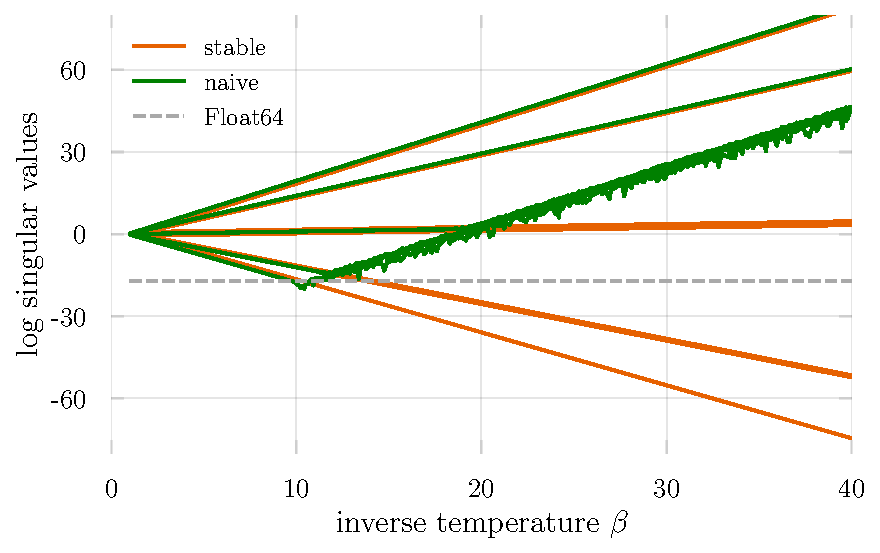
\includegraphics[width=0.45\textwidth]{figures/naive_vs_stable.pdf}
	\caption{\textbf{Numerical instabilities} (green) due to finite machine precision (\texttt{Float64}) in the calculation of the slice matrix product chain $B_M B_{M-1} \cdots B_1$ for model~\eqref{eq:model}. \label{fig:naive_vs_stable}}
\end{figure}

\begin{figure}[t]
	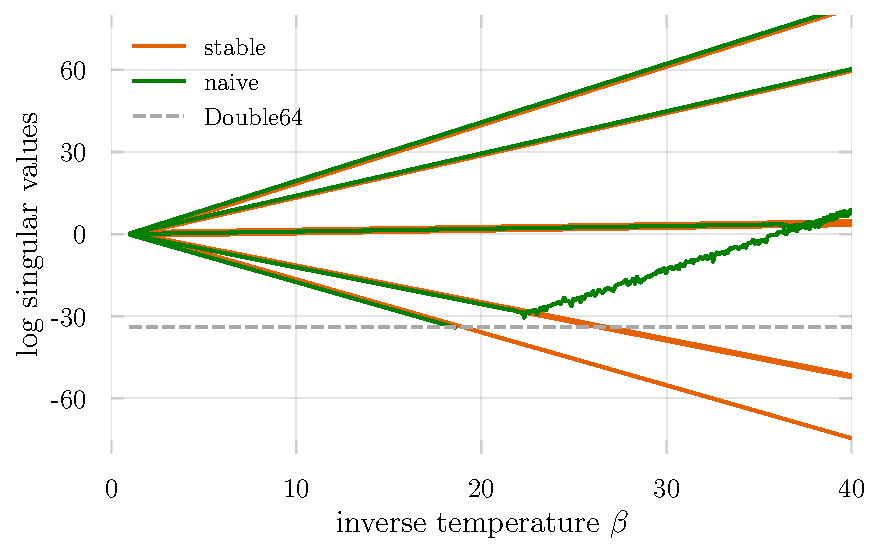
\includegraphics[width=0.45\textwidth]{figures/naive_vs_stable_db64.pdf}
	\caption{\textbf{Numerical instabilities} due to finite machine precision (\texttt{Double64}) in the calculation of the slice matrix product chain $B_M B_{M-1} \cdots B_1$ for model~\eqref{eq:model}. \label{fig:naive_vs_stable_db64}}
\end{figure}

\section{\label{sec:stabilization}Stabilization schemes}

One way to solve all problems is to switch to arbitrary precision numerics. In Julia the latter is provided through the \texttt{BigFloat} data type. However, this comes at the expense of (very) slow performance since, among other things, \texttt{BigFloat} lacks hardware support. Arbitrary precision numerics is still a valuable tool and we will use it to benchmark the accuracy of stabilization methods below.

How can we remedy the numerical issue outlined above in a floating point precision computation? The idea is to keep different scales separated throughout the computation as long as possible and only mix them in the final step, if necessary. A way to realize this is by deploying matrix decompositions, which we write generally as
\begin{align}
	B = UDX.
\end{align}
Here, $U$ and $X$ are matrices containing scales of the order of unity and $D$ is a real diagonal matrix having all the scales of $B$ separated on the diagonal. We will refer to the values in $D$ as singular values for all particular decompositions.

Instead of calculating the matrix product $B_2 B_1$ directly, we safely compute (\texttt{fact\_mult} in \texttt{StableDQMC.jl})

\begin{align}
B_2 B_1 &= \underbrace{U_2 D_2 X_2}_{B_2}\underbrace{U_1 D_1 X_1}_{B_1} \nonumber\\
&= U_2 \underbrace{(D_2 ((X_2 U_1) D_1))}_{U' D' X'} X_1)\\
&= U_r D_r X_r, \nonumber
\end{align}
with $U_r = U_2 U'$, $D_r = D'$, and $X_r = X' X_1$. Here, brackets indicate the order of operations. If we follow this scheme, largely different scales contained in the diagonal matrices won't be mixed throughout the computation. Repeating this procedure for the full slice matrix product chain, Eq.~\eqref{eq:Bchain}, we obtain an accurate $UDX$ decomposition of the result.\footnote{Note that we intentionally do not discuss the option to calculate $B^M$ as $U D^M X$ since typically the system will be interacting and the $B$ matrices in the product chain will differ.} \textcolor{red}{TODO: Mention safe mult}

Using this scheme, we have to be careful to keep different scales separated in the equal-time Green's function calculation, Eq.~\ref{etgf}, as well. A straightforward procedure (\texttt{inv\_one\_plus} in \texttt{StableDQMC.jl}) to add the unit matrix and perform the inversion in a stabilized manner is given by\cite{Santos2003, Assaad2002a}

\begin{align}
	G &= [\mathbb{1} + UDX]^{-1} \nonumber \\
	&= [U\underbrace{(U^\dagger X^{-1} + D)}_{udx}X]^{-1} \nonumber\\
	&= [(Uu)d(xX)]^{-1} \label{eq:inversion}\\
	&= U_r D_r X_r \nonumber,
\end{align}
with $U_r = (xX)^{-1}$, $D_r = d^{-1}$, $X_r = (Uu)^{-1}$.

Another prescription for a stabilized inversion (\texttt{inv\_one\_plus\_loh} in \texttt{StableDQMC.jl}), where we initially separate the scales in as $D_p = \max(D, 1)$ and $D_m = \min(D, 1)$ and perform two intermediate decompositions, is given by\cite{Loh2005, Loh1989}
\begin{align}
	G &= [\mathbb{1} + UDX]^{-1} \nonumber\\
	&= [(D_p^{-1} X^{-1} + U D_m) D_p X]^{-1} \nonumber \\
	&= X^{-1} \underbrace{[D_p^{-1} (\underbrace{D_p^{-1} X^{-1} + UD_m}_{udx})^{-1}]}_{udx} \label{eq:inversion_loh} \\
	&= U_r D_r X_r, \nonumber
\end{align}
with $U_r = X^{-1}u$, $D_r = d$, and $X_r = x$. We will demonstrate below that it is sometimes necessary to employ this second procedure to obtain accurate results for $G$.\\

So far we haven't specified a concrete decomposition $B = UDX$. In fact, there are a couple of choices, two of which we will focus on in what follows.

\subsection{SVD ($UDV^\dagger$)}
A SVD is given by
\begin{align}
	B = USV^\dagger,
\end{align}
where $U$ is unitary, $S$ is a real diagonal matrix, and $V^\dagger$ is unitary. In this case we can use the unitarity of $U$ and $V^\dagger$ to calculate inverse terms like, for example, $(Uu)^{-1}$ in the last line of \ref{eq:inversion} as $(Uu)^{-1} = u^\dagger U^\dagger$, which is generally cheaper.

Julia offers a couple of purely-Julia SVD implementations, like \href{https://github.com/JuliaLinearAlgebra/GenericSVD.jl/}{GenericSVD.jl}, which we will use for \texttt{BigFloat} computations. However, some of the most optimized algorithms are part of LAPACK\cite{LAPACK} and Julia defaults to those algorithms for regular floating point types. Concretely, there are three SVD functions\footnote{Note that Fortran LAPACK functions are named according to realness and symmetries of the matrix. In Julia multiple-dispatch takes care of routing different matrix types to different \textit{methods}. The Julia function \texttt{gesdd} works for both real and complex matrices, i.e. there is no (need for) \texttt{cgesdd}.} implementing different algorithms for calculating the SVD:
\begin{itemize}
	\item \texttt{gesdd} (default): Divide-and-conquer (D\&C)
	\item \texttt{gesvd}: Conventional
	\item \texttt{gesvj}: Jacobi algorithm (through \href{https://github.com/RalphAS/JacobiSVD.jl}{JacobiSVD.jl})
\end{itemize}
which can be readily accessed via convenience wrappers of the same name exported by \texttt{StableDQMC.jl}. We will compare all of them below.

\subsection{QR ($UDT$)}
A QR decomposition reads
\begin{align}
B = QR = UDT,
\end{align}
where we have split $R$ into a diagonal, $D$, and upper triangular piece $T$. Hence, $U = Q$ is unitary, $D = \textrm{diag}(R)$ is a real diagonal matrix, and $T$ is upper triangular. In Julia, one can obtain the $QR$ factored form of a matrix by calling the function \texttt{qr} from the standard library \texttt{LinearAlgebra}. The splitting into $UDT$ form is provided by \texttt{udt} and \texttt{udt!} in in \texttt{StableDQMC.jl}.

\section{Benchmarks}

In the following we want to assess how the mentioned matrix decompositions perform in stabilized computations of the slice matrix product chain $B_M \cdots B_1$, the Green's function $G$, and it's determinant $\det G$, both with respect to accuracy and speed, for our model system in Eq.~\ref{eq:model}.

\subsection{Accuracy}

\begin{figure}
	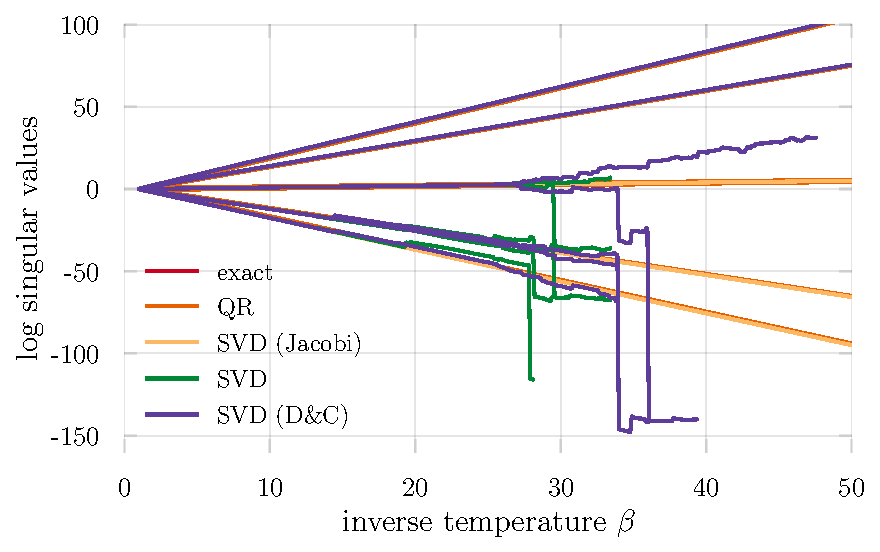
\includegraphics[width=0.45\textwidth]{figures/decomp_comparison_simple.pdf}
	\caption{\textbf{Comparison of matrix decompositions} to heal the numerical instabilities in the calculation of the slice matrix product chain $B_M B_{M-1} \cdots B_1$ for model~\eqref{eq:model}. The QR and Jacobi SVD singular values seem to lie on top of the exact ones whereas regular SVD and divide-and-conquer SVD show large deviations at low temperatures $\beta \gtrsim 25$ ($\Delta \tau = 0.1$). \label{fig:decomp_comparison_simple}}
\end{figure}

Before benchmarking the efficiency of an algorithm, it is crucial to check it's correctness first. Fig.~\ref{fig:decomp_comparison_simple} shows the log singular values of the slice matrix product chain Eq.~\ref{eq:Bchain} stabilized with different matrix decompositions as a function of it's length $M$. While QR and Jacobi SVD seem to lie on top of the numerically exact result, we observe large deviations for the simple and D\&C SVD algorithms at low temperatues ($\beta \gtrsim 25)$.\footnote{\textcolor{red}{LAPACK SVD error bounds\cite{errorbounds} '\textit{Thus large singular values (those near $\sigma_1$) are computed to high relative accuracy and small ones may not be.}'}}\\

\begin{figure}[t]
	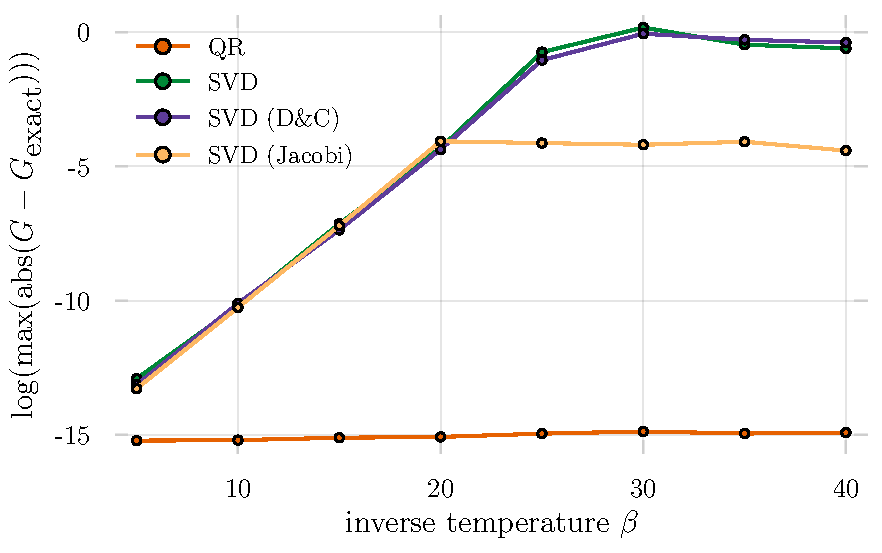
\includegraphics[width=0.45\textwidth]{figures/accuracy_greens_svd_regularinv.pdf}
	\caption{\textbf{Accuracy of the Green's function} obtained from stabilized computations using the listed matrix decompositions and the inversion scheme \texttt{inv\_one\_plus}, Eq.~\eqref{eq:inversion}. \label{fig:greens_accuracy_regularinv}}
\end{figure}

\begin{figure}[t]
	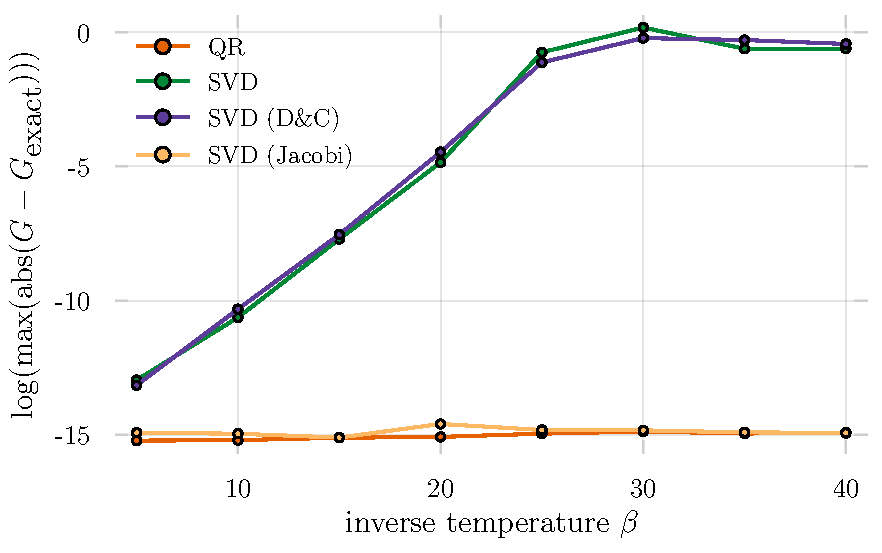
\includegraphics[width=0.45\textwidth]{figures/accuracy_greens_svd_loh.pdf}
	\caption{\textbf{Accuracy of the Green's function} obtained from stabilized computations using the listed matrix decompositions and the careful inversion scheme \texttt{inv\_one\_plus\_loh}, Eq.~\ref{eq:inversion_loh}. \label{fig:greens_accuracy_loh}}
\end{figure}

Turning to the equal-time Green's function, Eq.~\eqref{etgf}, we take the results for the slice matrix chains and perform the inversions according to the schemes presented above. We take the maximum absolute difference between the obtained Green's functions and the exact $G$ as an accuracy measure. The findings for the simple inversion scheme \texttt{inv\_one\_plus}, Eq.~\ref{eq:inversion}, are shown in Fig.~\ref{fig:greens_accuracy_regularinv}. At high temperatures, all decompositions give the correct Green's function up to some limit close to floating point precision. However, at low temperatures only the QR decomposition reproduces $G_{\textrm{exact}}$ reliably. It has the highest accuracy by a large margin, followed by the Jacobi SVD as the best of the SVD methods, which all fail to reproduce the exact result accurately. As displayed in Fig.~\ref{fig:greens_accuracy_loh}, switching to the more careful procedure \texttt{inv\_one\_plus\_loh}, Eq.~\ref{eq:inversion_loh}, does improve the accuracy of the Jacobi SVD dramatically while the deviations seen for the other two SVD based schemes are still of order unity.
\begin{figure}
	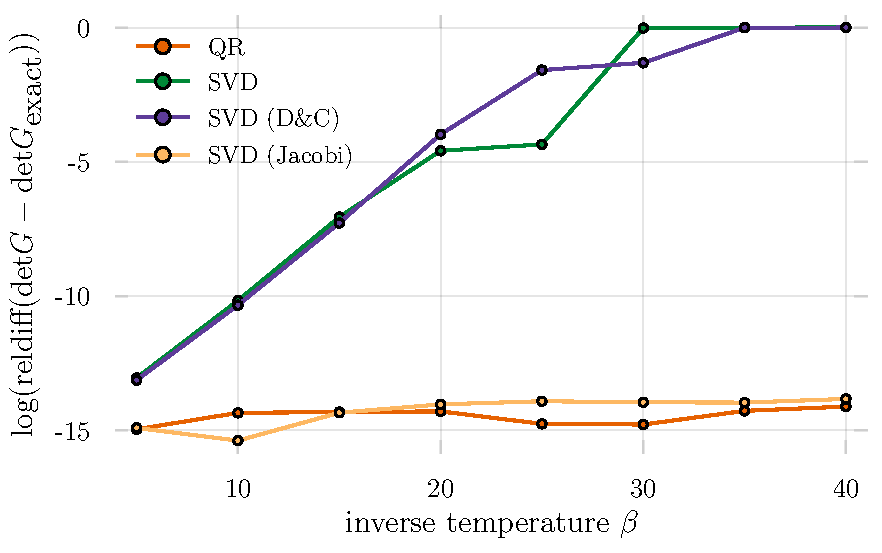
\includegraphics[width=0.45\textwidth]{figures/accuracy_det_svd_regularinv.pdf}
	\caption{\textbf{Accuracy of the determinant} of the equal-time Green's function obtained from stabilized computations using the listed matrix decompositions and the inversion scheme \texttt{inv\_one\_plus}, Eq.~\ref{eq:inversion}. \label{fig:det_accuracy_regularinv}}
\end{figure}

\begin{figure}
	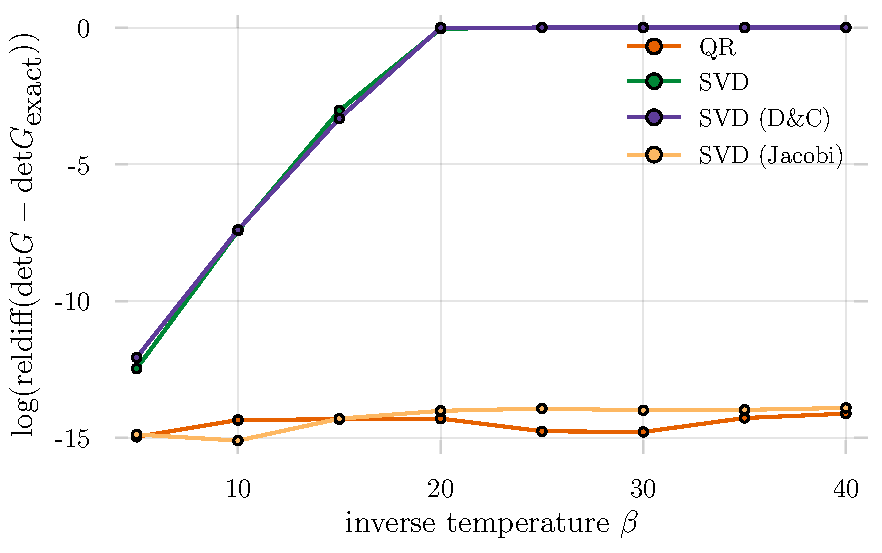
\includegraphics[width=0.45\textwidth]{figures/accuracy_det_svd_loh.pdf}
	\caption{\textbf{Accuracy of the determinant} of the equal-time Green's function obtained from stabilized computations using the listed matrix decompositions and \texttt{inv\_one\_plus\_loh}, Eq.~\ref{eq:inversion_loh}. \label{fig:det_accuracy_loh}}
\end{figure}

In Figs.~\ref{fig:det_accuracy_regularinv},~\ref{fig:det_accuracy_loh} we show the logarithm of the relative error of the Green's function determinant, relevant in the Metropolis acceptance\footnote{For local updates on can generally avoid full calculations of Green's function determinants by exploiting locality and performing a Laplace expansion since only ratios of determinants appear in Eq.~\ref{eq:metropolis}. In fact, in an optimal implementation the computation of the acceptance rate is $O(1)$ rather than $O(N^3)$.}, obtained for all combinations of matrix decompositions and inversion schemes. Both the QR decomposition and the Jacobi SVD lead to accurate results for all accessed temperatures, irrespective of the employed inversion scheme. The other two SVD based methods on the other hand show large relative deviations for both \texttt{inv\_one\_plus} and \texttt{inv\_one\_plus\_loh}.

These findings suggest that only the QR decomposition, independent of the inversion procedure, or the Jacobi SVD in combination with the more careful inversion scheme \texttt{inv\_one\_plus\_loh} is suited for computing both the equal time Green's function and it's determinant reliably.

%\begin{table}[b]
%	\bgroup
%	\def\arraystretch{1.25}%  1 is the default, change whatever you need
%	\begin{tabular}{ccc}
%		$\beta = 5$ & Method & $\textrm{max}(\textrm{abs}(G - G_{\textrm{exact}}))$ \\
%		\hline
%		& QR & 6.1e-16 \\ 
%
%		& SVD, simple & 8.1e-14 \\ 
%
%		& SVD, D\&C & 6.9e-14 \\ 
%
%		& SVD, Jacobi & 6.1e-14 \\ 
%		\hline
%		& \\ 
%		$\beta = 40$ & Method & $\textrm{max}(\textrm{abs}(G - G_{\textrm{exact}}))$ \\
%		\hline
%		
%		& QR & 1.2e-15 \\ 
%
%		& SVD, simple & 4.7e-1 \\ 
%
%		& SVD, D\&C & 4.9e-1 \\ 
%
%		& SVD, Jacobi & 3.1e-4 \\ 
%		\hline
%	\end{tabular}
%	\egroup
%	\caption{\textbf{Accuracy of the Green's function} obtained from stabilized computations using the listed matrix decompositions at high ($\beta = 5$) and low temperatures ($\beta = 40$). \label{tbl:greens_accuracy}}
%\end{table}




%\begin{table}
%	\bgroup
%	\def\arraystretch{1.25}%  1 is the default, change whatever you need
%	\begin{tabular}{cccc}
%		$\beta = 5$ & Method & $\Delta_\textrm{abs} (\textrm{det} G)$ & $\Delta_\textrm{rel}(\textrm{det} G)$ \\
%		\hline
%		& QR & 2.3e-27 & 1.1e-15 \\ 
%		
%		& SVD, simple & 3.2e-26 & 1.5e-14 \\ 
%		
%		& SVD, D\&C & 1.8e-25 & 8.5e-14 \\ 
%		
%		& SVD, Jacobi & 1.2e-25 & 5.7e-14 \\ 
%		\hline
%		& \\ 
%		$\beta = 40$ & Method & $\Delta_\textrm{abs}(\textrm{det} G)$ & $\Delta_\textrm{rel}(\textrm{det} G)$ \\
%		\hline
%		
%		& QR & 4.1e-107 & 7.7-15 \\ 
%		
%		& SVD, simple & 4.5e-90 & 1.0e-0 \\ 
%		
%		& SVD, D\&C & 2.6e-93 & 1.0e-0 \\ 
%		
%		& SVD, Jacobi & 8.8e-97 & 1.7e-4 \\ 
%		\hline
%	\end{tabular}
%	\egroup
%	\caption{\textbf{Accuracy of the determinant} of the equal-time Green's function obtained from stabilized computations using the listed matrix decompositions at high ($\beta = 5$) and low temperatures ($\beta = 40$). \label{tbl:det_accuracy}}
%\end{table}



\subsection{Efficiency}



%\afterpage{\clearpage}
\section{Time-displaced Green's function}
\citet{Loh2005} method
Hirsch method\cite{Hirsch1988}

We generalize our definition of the equal times Green's function, Eq.~\ref{etgf}, to include the imaginary time $\tau = l \Delta \tau$ dependence,
\begin{align}
G(\tau) = \langle c_{i} c_{j}^\dagger \rangle_{\phi_l} = \left( 1 + B_{l-1}\dots B_1 B_M \dots B_l \right)^{-1}.
\end{align}
Note that $ G \equiv G_1 = G_{M+1} = \left( 1 + B_M \dots B_l \right)^{-1} $. The time displaced Green's function can now be defined as\cite{Santos2003, Assaad2002a}
\begin{align*}
	G_{l_1,l_2} &\equiv G(\tau_1, \tau_2) \equiv \langle T c_i(\tau_1) c_j^\dagger(\tau_2) \rangle_\varphi,
\end{align*}
where $T$ represents time ordering.

More explicitly this reads
\begin{align}
	G(\tau_1, \tau_2) = \begin{cases}
	B_{l_1} \cdots B_{l_2 + 1} G_{l_2 + 1}, &\tau_1 > \tau_2,\\
	- \left( 1 - G_{l_1 + 1} \right) \left( B_{l_2} \cdots B_{l_1 + 1}\right)^{-1}, &\tau_2 > \tau_1.
	\end{cases} \label{eq:tdgf_propagate}
\end{align}
In principle, this gives us a prescription for how to calculate $G(\tau_1, \tau_2)$ from the equal time Green's function $G(\tau)$ (which we know how to stabilize). However, when $|\tau_1 - \tau_2|$ is large a naive calculation of slice matrix product chains in Eq.~\ref{eq:tdgf_propagate} would be numerically unstable, as seen above. Also, by first calculating $G$ we already mix important scale information in the last recombination step, in which we multiply $G = UDX$. We therefore rather compute the time-displaced Green's function directly as
\begin{align}
	G(\tau_1, \tau_2) = (U_L D_L X_L + U_R D_R X_R)^{-1}.
\end{align}
Similar to Sec.~\ref{sec:stabilization}, we must be very careful to keep the involved scales separated as much as possible when performing the summation and the inversion.
As a first explicit procedure, we consider a simple generalization of Eq.~\ref{eq:inversion} (\texttt{inv\_sum} in \texttt{StableDQMC.jl}),
\begin{align}
	G(\tau_1, \tau_2) &= [U_L D_L X_L + U_R D_R X_R]^{-1} \nonumber\\
	&= [U_L \underbrace{(D_L X_L X_R^{-1} + U_L^\dagger U_R D_R)}_{udx} X_R ]^{-1} \nonumber\\
	&= [(U_L u) d^{-1} (x X_R)]^{-1} \\
	&= U_r D_r X_r, 
\end{align}
where $U_r = (x X_R)^{-1}$, $D_r = d^{-1}$, and $X_r = (U_L u)^{-1}$.

Another scheme, analogous to Eq.~\ref{eq:inversion_loh}, where we split the scales in $D$, is as follows (\texttt{inv\_sum\_loh} in \texttt{StableDQMC.jl}),
\begin{align}
	G(\tau_1, \tau_2) &= [U_L D_L X_L + U_R D_R X_R]^{-1} \nonumber\\
	&= [U_L D_{Lm} D_{Lp} X_L + U_R D_{Rm} D_{Rp} X_R]^{-1} \nonumber\\
	&= \left[U_L D_{Lp} \underbrace{\left( \dfrac{D_{Lm}}{D_{Rp}} X_L X_R^{-1} + U_L^\dagger U_R \dfrac{D_{Rm}}{D_{Lp}} \right)}_{udx} X_R D_{Rp} \right]^{-1} \nonumber\\
	&= X_R^{-1} \underbrace{\dfrac{1}{D_{Rp}} [udx]^{-1} \dfrac{1}{D_{Lp}}}_{udx} U_L^\dagger \\
	&= U_r D_r X_r,
\end{align}
with $U_r = X_R^{-1} u$, $D_r = d$, and $X_r = x U_L^\dagger$.







%\afterpage{\clearpage}
\clearpage
\bibliography{references}
%\clearpage
%\appendix


\end{document}
%
% ****** End of file apssamp.tex ******
